\newpage

\section{Experiments: PseudoCylindrical projections}
\subsection{Robinson}
\begin{figure}[H]
    \centering
    \begin{minipage}{0.30\textwidth}
        \centering
        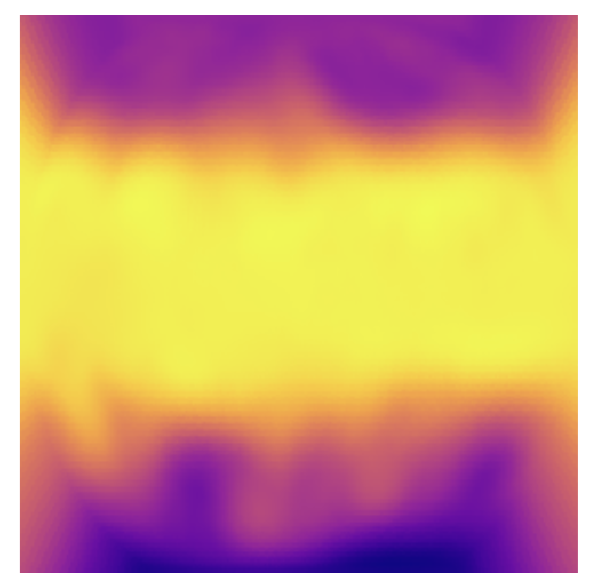
\includegraphics[width=0.9\linewidth]{figures/chapter-8/geopoth_robin.png}
        \caption{ Geopotential height raster data as Robinson projected}
        \label{fig:robin_geopoth_raster}
    \end{minipage}\hfill
    \begin{minipage}{0.30\textwidth}
        \centering
        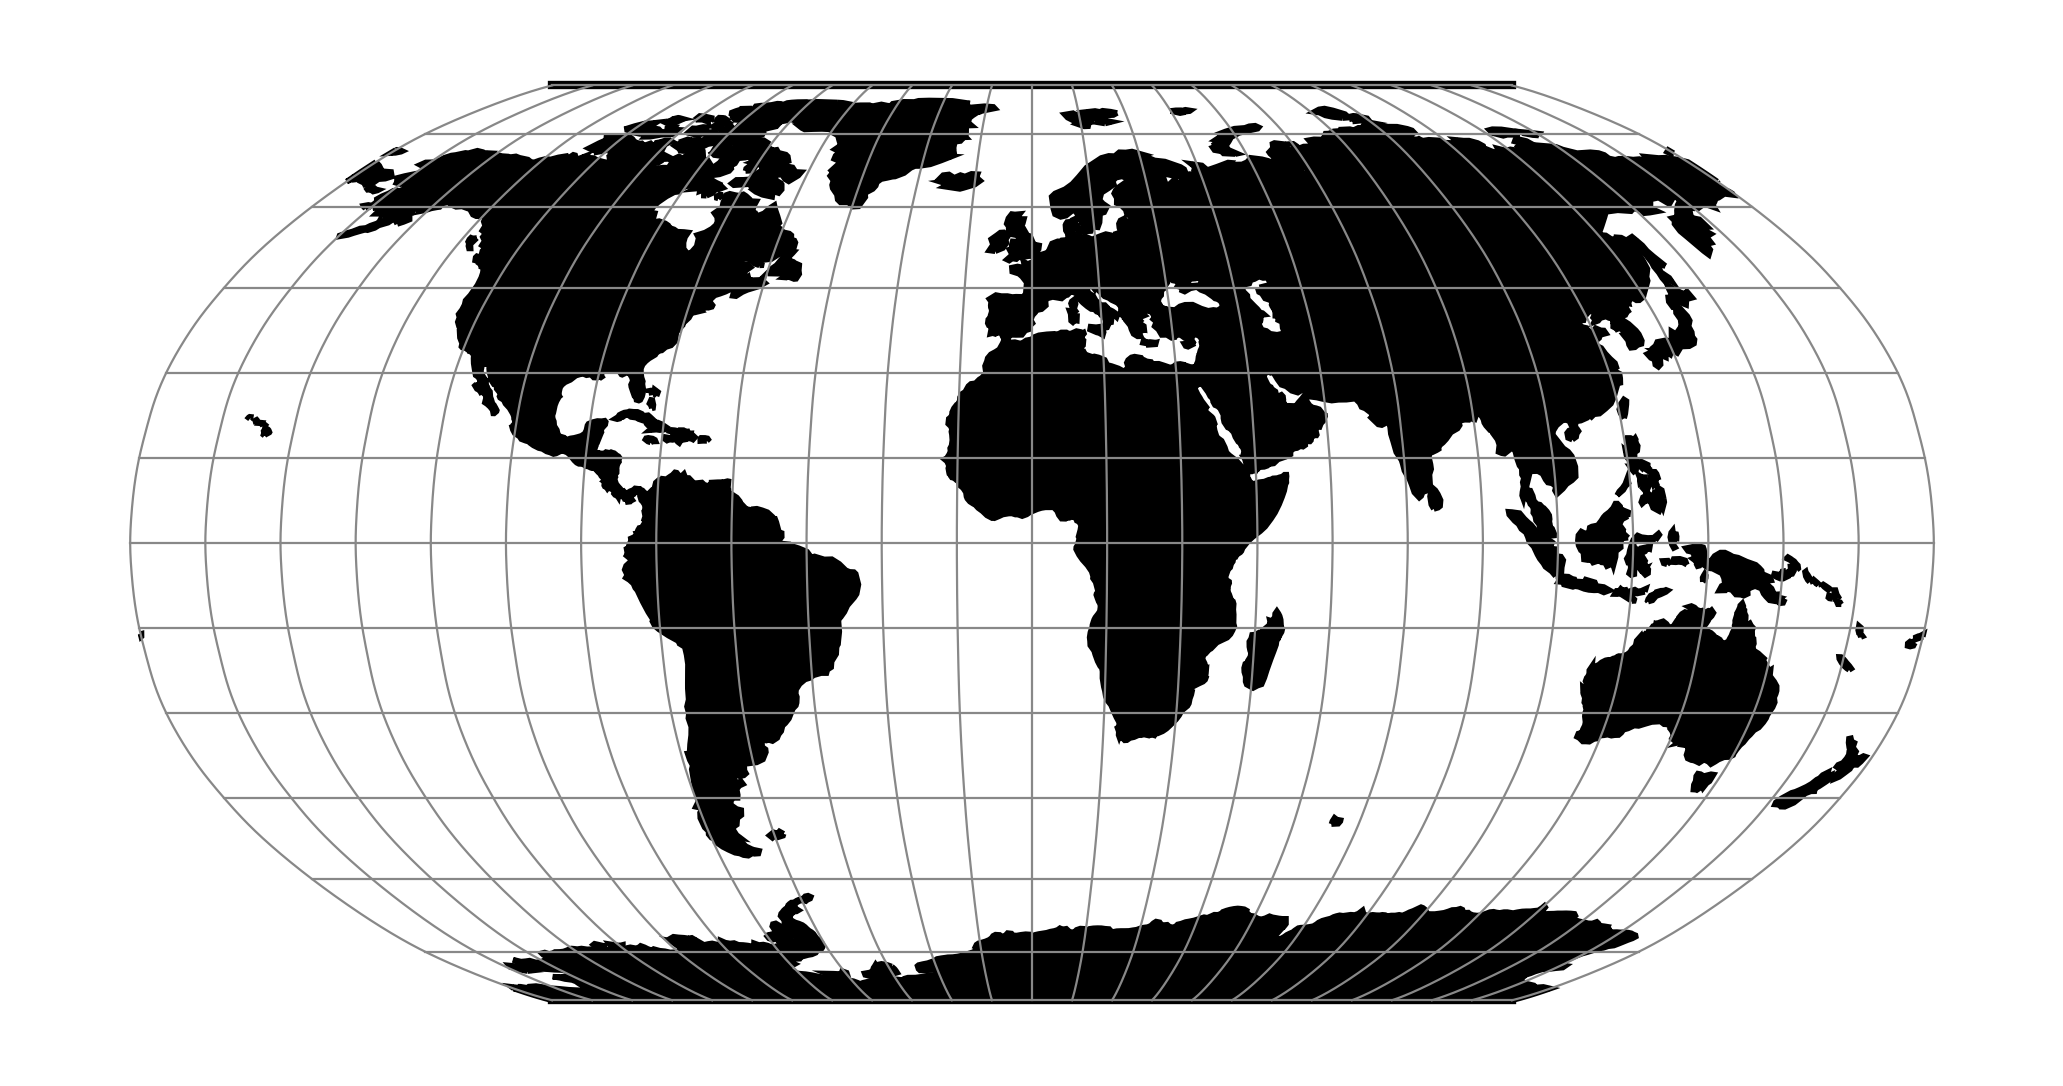
\includegraphics[width=0.9\linewidth]{figures/chapter-8/robin.png}
        \caption{Robinson (Source \cite{PROJ_SITE})}
        \label{fig:robin_proj}
    \end{minipage}\hfill
    \begin{minipage}{0.30\textwidth}
        \centering
        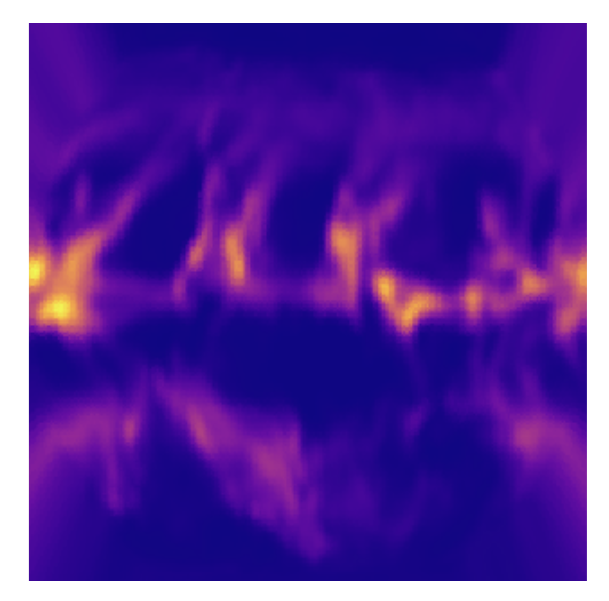
\includegraphics[width=0.9\linewidth]{figures/chapter-8/prect_robin.png}
        \caption{Precipitation raster data as Robinson projected}
        \label{fig:robin_prect_raster}
    \end{minipage}\hfill
\end{figure}
\begin{figure}[H]
    \centering
    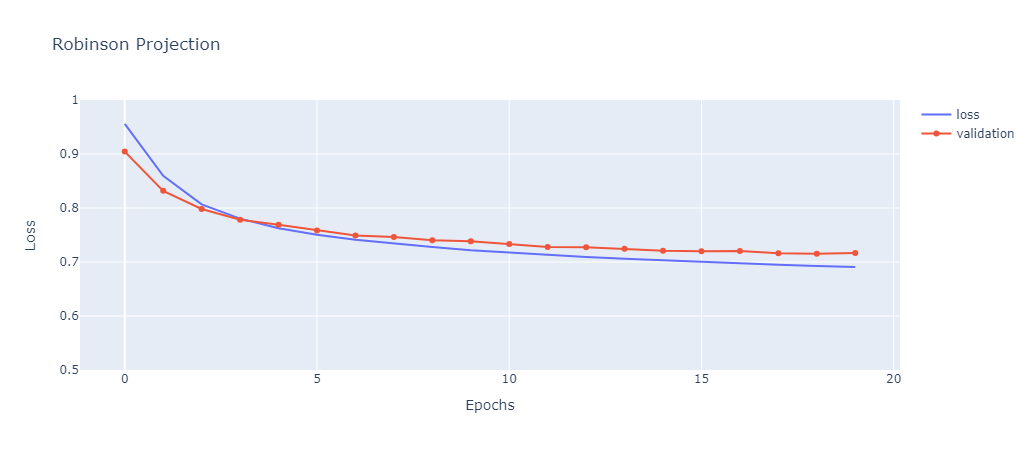
\includegraphics[width=1.0\linewidth]{figures/chapter-8/robin_loss.png}
    \caption{Robinson: Averaged training loss of models  }
    \label{fig:robin_loss}
\end{figure}
\subsection{Interrupted Goode Homolosine}
\begin{figure}[h]
    \centering
    \begin{minipage}{0.30\textwidth}
        \centering
        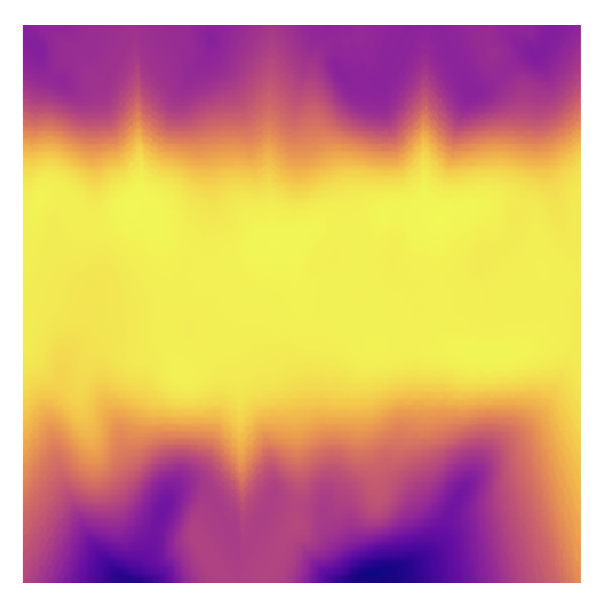
\includegraphics[width=0.9\linewidth]{figures/chapter-8/geopoth_goode.png}
        \caption{ Geopotential height raster data as Interrupted Goode Homolosine projected}
        \label{fig:ig_geopoth_raster}
    \end{minipage}\hfill
    \begin{minipage}{0.30\textwidth}
        \centering
        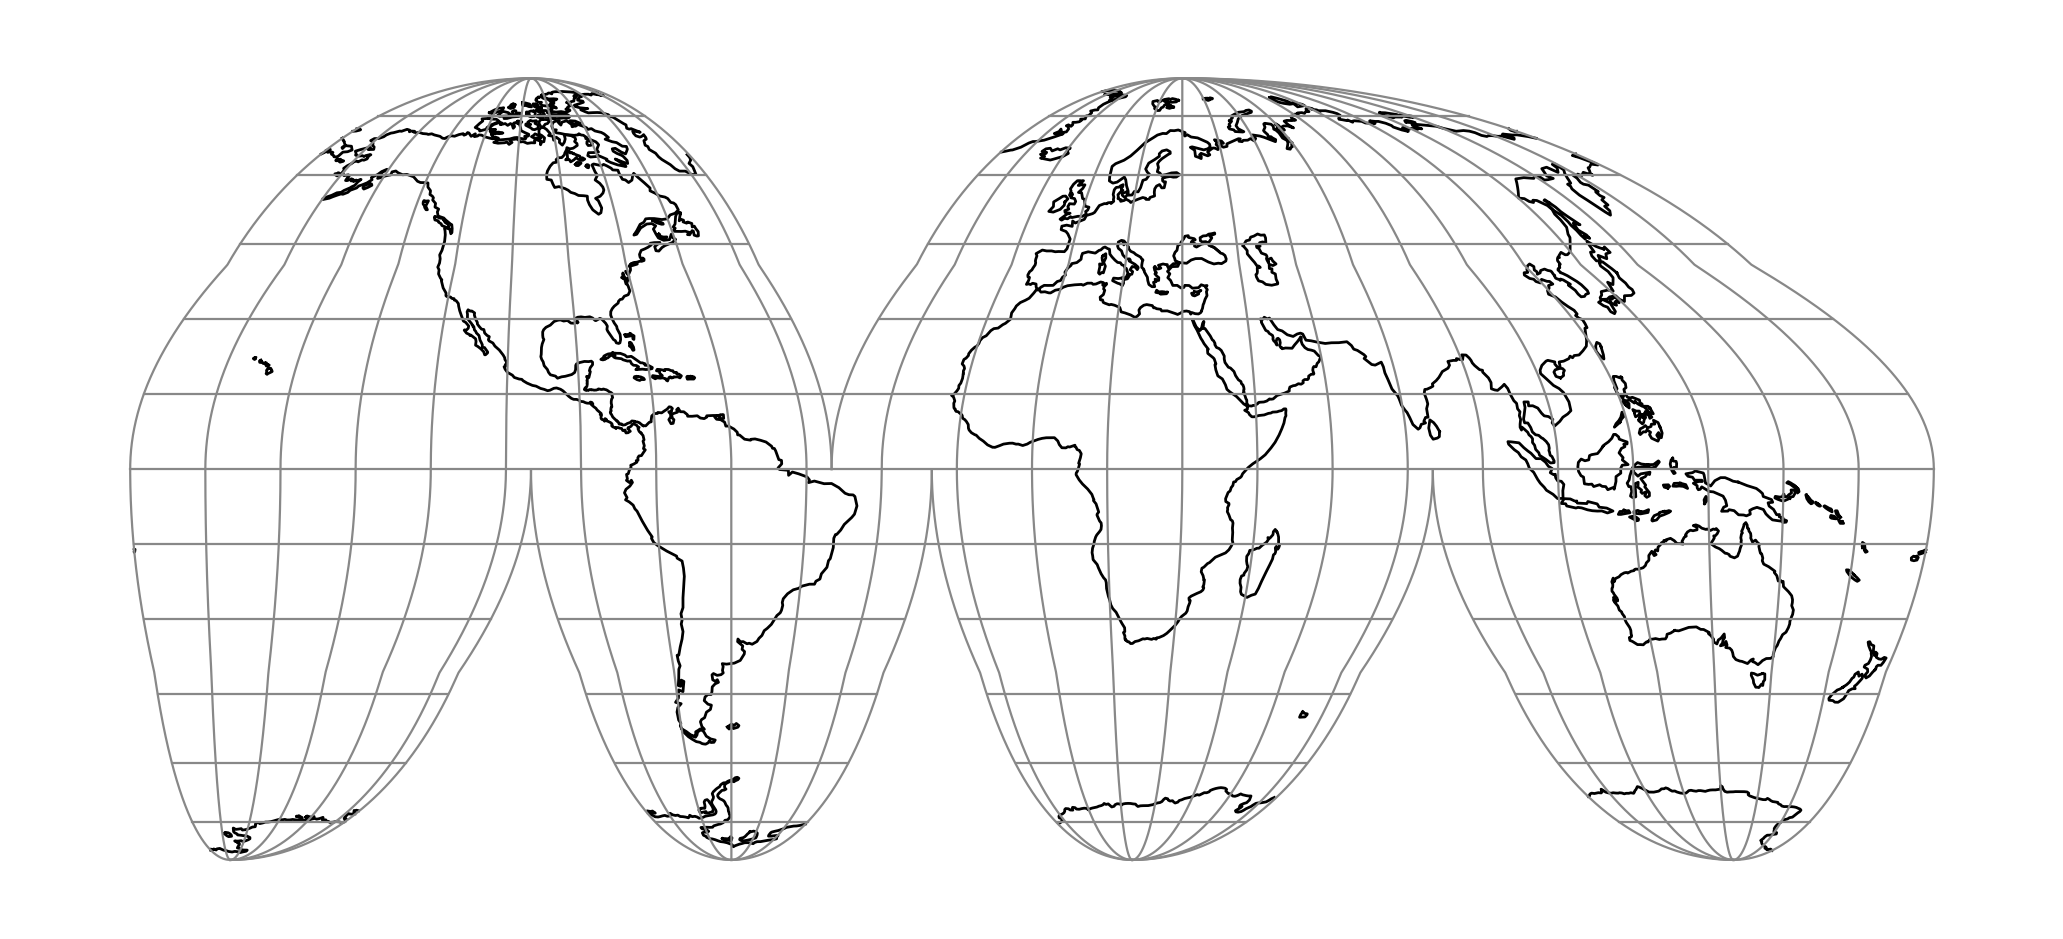
\includegraphics[width=0.9\linewidth]{figures/chapter-8/igh.png}
        \caption{Interrupted Goode Homolosine (Source \cite{PROJ_SITE})}
        \label{fig:ig_proj}
    \end{minipage}\hfill
    \begin{minipage}{0.30\textwidth}
        \centering
        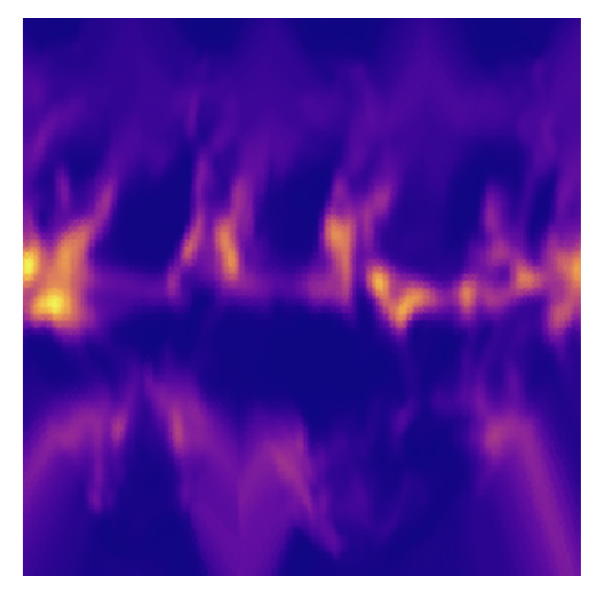
\includegraphics[width=0.9\linewidth]{figures/chapter-8/prect_goode.png}
        \caption{Precipitation raster data as Interrupted Goode Homolosine projected}
        \label{fig:ig_prect_raster}
    \end{minipage}\hfill
\end{figure}

\begin{figure}[H]
    \centering
    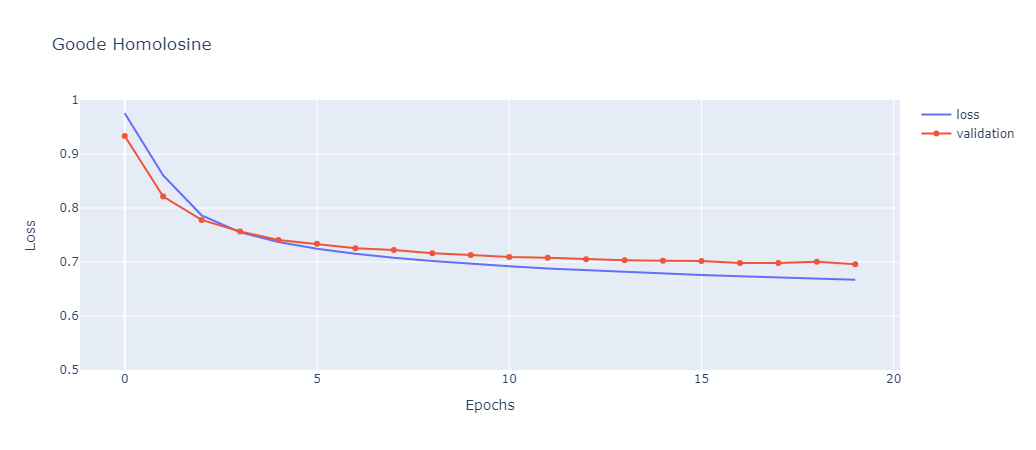
\includegraphics[width=1.0\linewidth]{figures/chapter-8/goode_loss.png}
    \caption{Interrupted Goode Homolosine: Averaged training loss of models  }
    \label{fig:goode_loss}
\end{figure}
\subsection{Sinusoidal Sanson Flamsteed}
\begin{figure}[H]
    \centering
    \begin{minipage}{0.30\textwidth}
        \centering
        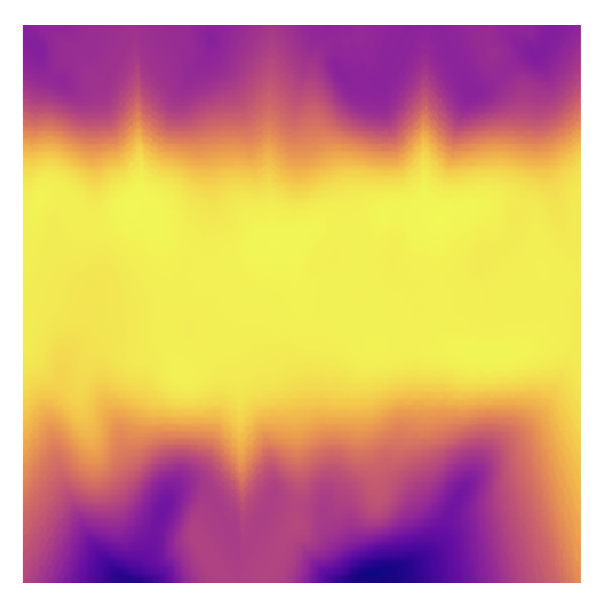
\includegraphics[width=0.9\linewidth]{figures/chapter-8/geopoth_goode.png}
        \caption{ Geopotential height raster data as Sinusoidal Sanson Flamsteed projected}
        \label{fig:ig_geopoth_raster}
    \end{minipage}\hfill
    \begin{minipage}{0.30\textwidth}
        \centering
        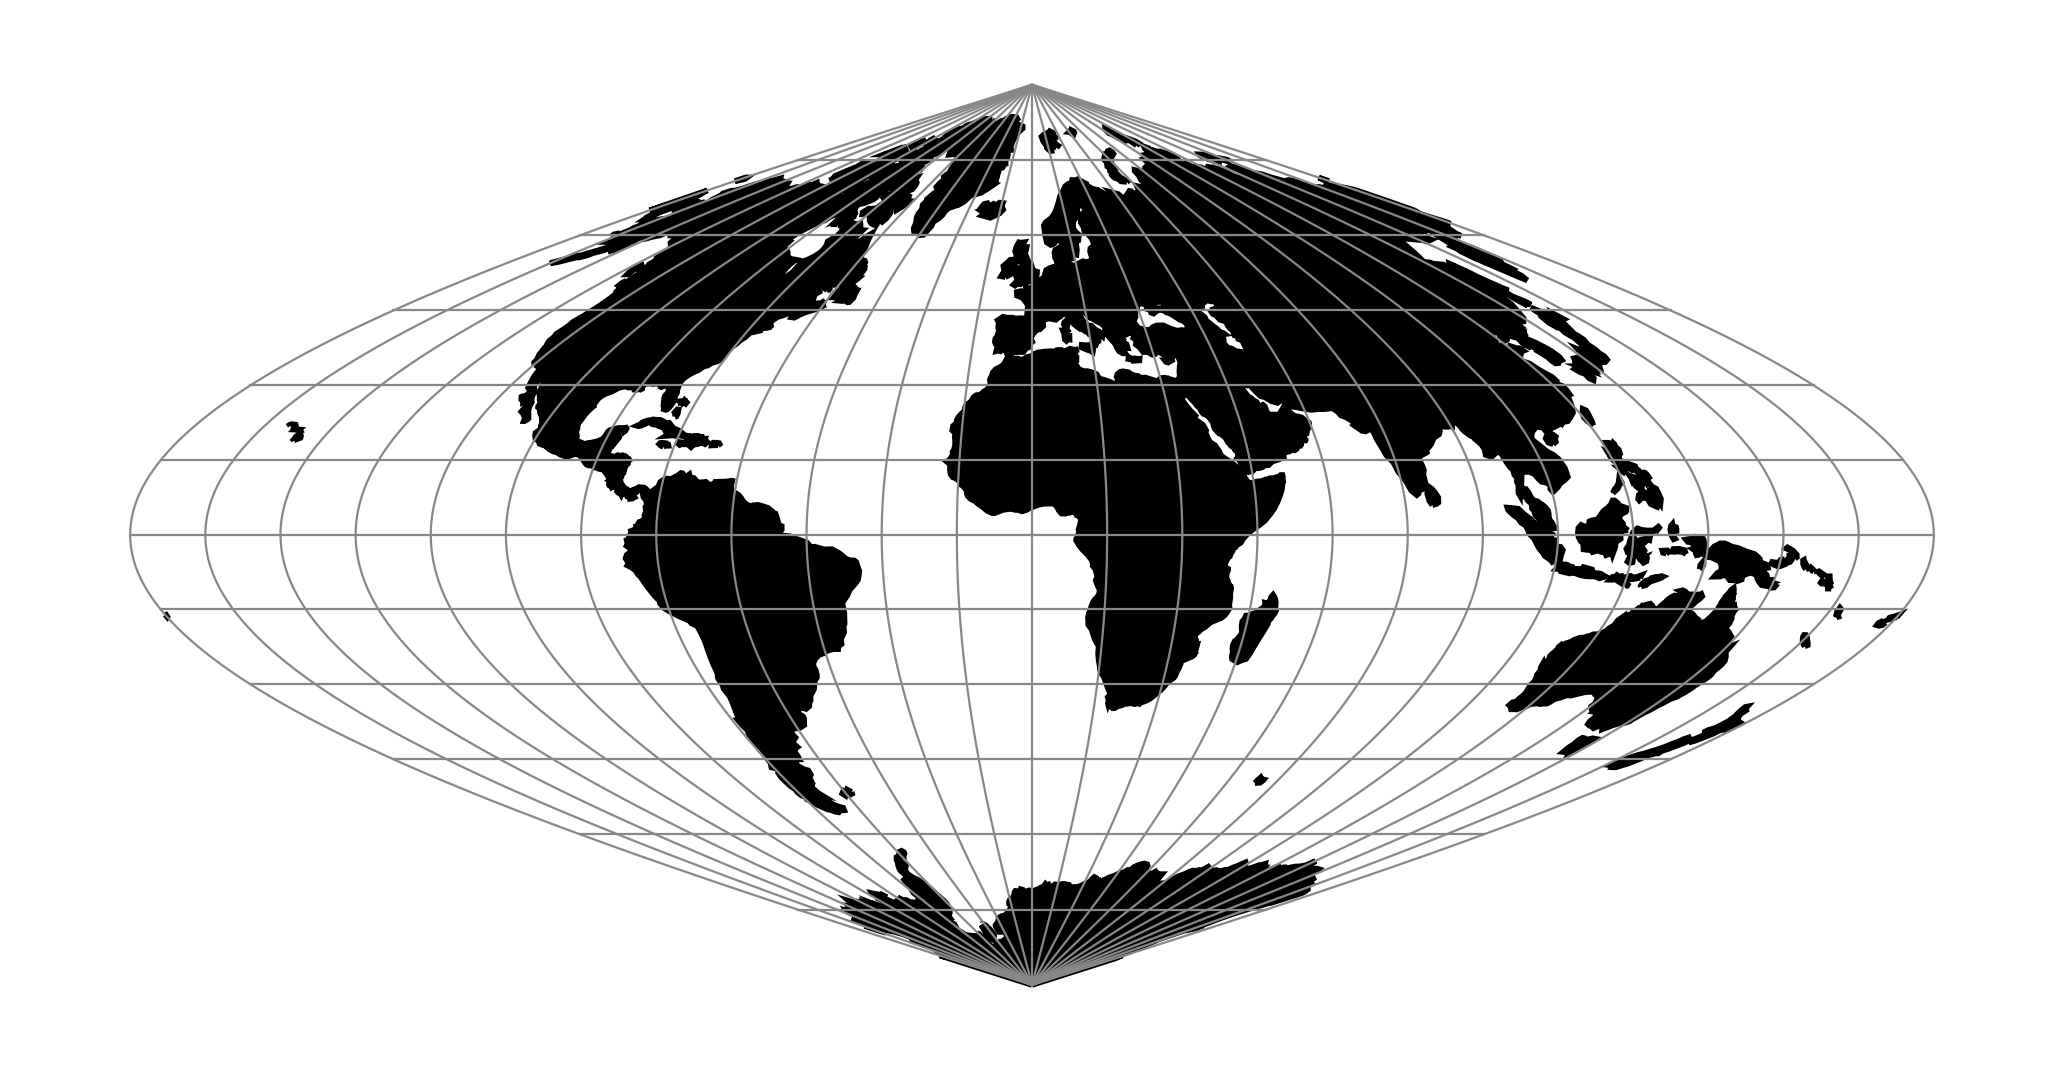
\includegraphics[width=0.9\linewidth]{figures/chapter-8/sinu.png}
        \caption{Sinusoidal Sanson Flamsteed (Source \cite{PROJ_SITE})}
        \label{fig:ig_proj}
    \end{minipage}\hfill
    \begin{minipage}{0.30\textwidth}
        \centering
        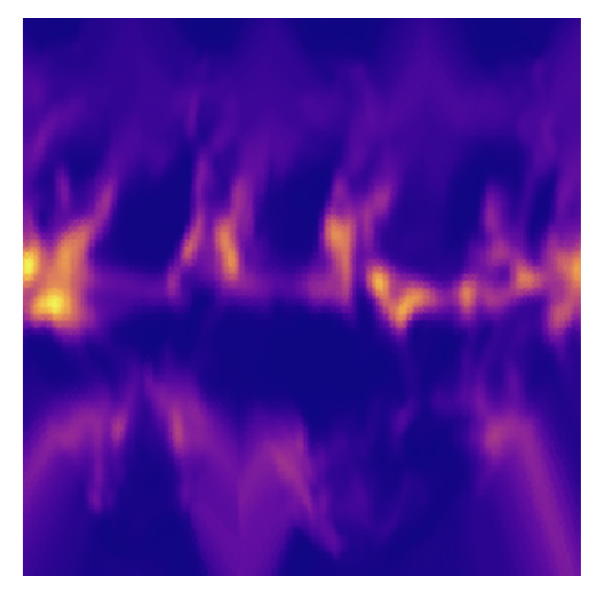
\includegraphics[width=0.9\linewidth]{figures/chapter-8/prect_goode.png}
        \caption{Precipitation raster data as Sinusoidal Sanson Flamsteed projected}
        \label{fig:ig_prect_raster}
    \end{minipage}\hfill
\end{figure}


\begin{figure}[H]
    \centering
    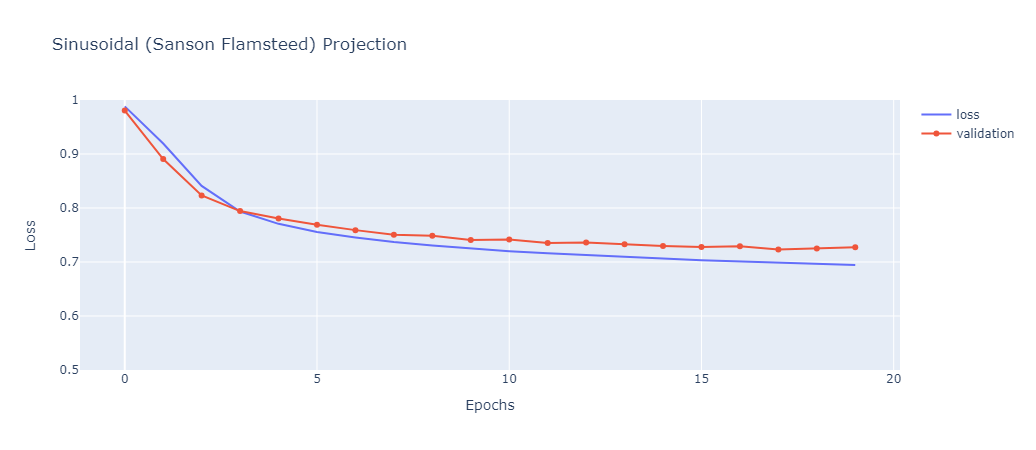
\includegraphics[width=1.0\linewidth]{figures/chapter-8/sinu_loss.png}
    \caption{Sinusoidal Sanson Flamsteed: Averaged training loss of models  }
    \label{fig:sinu_loss}
\end{figure}


\subsection{Results and Observations}
\begin{itemize}
    \item The Figures \ref{fig:robin_loss} \ref{fig:goode_loss} \ref{fig:sinu_loss} depict the training loss for the 3 of the 4 pseudocylindrical projections, the training and the validation loss value starts from a very high value of 1. All of the models are trended towards the overfitting trend,
          but the loss values are not decreasing as compared to the cylindrical projections.
    \item The overfitting trends are occuring in the robinson projection at epoch 8.
    \item The trend of overfitting in goode homolosine projected data is at epoch 7 and for the sinusoidal model it is on the 4th epoch.
    \item For the loximuthal projection the loss value is 0.690 and the validation loss is 0.716, even this projection is subjected to overfitting.
    \item It is the same phenomenon which was happening in the cylindrical projections when the data is spread on the whole raster, the model is overfitting, this projection is very much similar to robinson projection.
    \item The results in the Table ~\ref{pseudo_cylindrical_results_table} for predictions as compared to cylindrical projections is worse.
\end{itemize}
\begin{table}[ht]
    \centering
    \caption{Summary of Pseudocylindrical Projection Model Performance}
    \label{pseudo_cylindrical_results_table}
    \renewcommand{\arraystretch}{1.2} % Adjusts the row height
    \begin{tabular}{|l|c|c|c|c|c|}
        \hline
        \rowcolor[gray]{0.9}
        \textbf{\emph{Projection}}   & \textbf{\emph{\# Epochs}} & \textbf{\emph{MAE}} & \textbf{\emph{Validation MAE}} \\ \hline
        Robinson                     & 20                        & 0.617               & 0.627                          \\ \hline
        Interrupted Goode Homolosine & 20                        & 0.606               & 0.617                          \\ \hline
        Sinusoidal Sanson Flamsteed  & 20                        & 0.624               & 0.641                          \\ \hline
        Loximuthal                   & 20                        & 0.628               & 0.636                          \\ \hline
    \end{tabular}
\end{table}
